%!TEX root = ../dokumentation.tex

\chapter{Kommunikation zwischen Bilderkennung und Roboter\footnote{besseren Namen einfallen lassen, der dem neuen Inhalt gerecht wird(Kommunikation und Umrechnung oder so}}
\label{cha:Kommunikation zwischen Bilderkennung und Roboter}
\section{Kommunikation}
Die Kommunikation zwischen dem Roboter und dem Airhockeyprogramm erfolgt über das Ethernet. Dabei haben wir uns für die Kommunikation über Sockets entschieden, da dies die gängigste Methode ist und sowohl von der Programmiersprache des Roboters als auch von Python beherrscht wird. Der Roboter fungiert dabei als Client der sich mit einem Server verbindet. Die PC mit der Roboter-KI ist in diesem Fall der Server. Es hat keinen besonderen Grund wieso wir das so rum getan haben. Dies kann genauso gut auch andersrum implementiert werden, also mit dem Roboter als Server und dem PC-Programm als Client. Wir hatten beide Variante ausgetestet und mehrfach zwischen beiden hin- und hergewechselt. Da wir aber bei unseren Tests keine Geschwindigkeitsunterschiede zwischen beiden feststellen konnten, haben wir dann letztenendes die oben genannte Variante einfach gelassen.

Mithilfe von Sockets wird eine Folge von Bytes übertragen. Da sowohl erweiterter ANSI-Code als auch UTF-8 ein Byte groß sind, könnte man diese Folge von Bytes auch als eine Folge von Zeichen interpretieren. Wie dies die jeweilige Programmiersprache interpretiert sollte man am besten im jeweiligen Handbuch nachlesen. In unseren Fall hat RAPID und Python 2.7 die übertragenen Daten als String angesehen, also als eine Folge von Zeichen. 
%Dies war recht gelegen, da dadurch keine komplizeirten Umformungen vorgenommen werden mussten. 
Übertragen wurde nur die Position, zu der sich der Roboter bewegen soll.  Da sich das Spielfeld nur auf einer 2-Dimensionalen Ebene befindet, waren dazu nur eine X- und Y-Koordinate nötig. Diese wurden durch ein Semikolon getrennt, wodurch die Daten wieder recht einfach auf Seite des Roboters getrennt werden konnten. Anfänglich war das nur eine Kommunikation in eine Richtung, wurde aber später noch ergänzt um eine Art \"Bereit\", das vom Roboter zurück gesendet wurde, sobald dieser seine Position erreicht hat und neue Befehle entgegennehmen kann. 

\section{Umrechnung vom Bildkoordinatensystem und Roboterkoordinatensystem}

\begin{wrapfigure}{R}{0pt}
	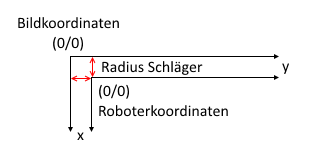
\includegraphics{Umrechnung_Koordinatensysteme.png}
	\vspace{-15pt}
	\caption{ Veranschaulichung der Koordinatensystemunterschiede}
	\label{img:Umrechnung Koordinatensysteme}
\end{wrapfigure}

Bilderkennung und Roboter nutzen unterschiedliche Koordinatensysteme. Das Bildkoordinatensystem enthält für die X- und Y"~Daten Werte von 0 bis 1. Dieses geht von einer Ecke (0/0) bis in die entgegengesetzte Ecke (1/1). Es verwendet ein normalisiertes Koordinatensystem. Es ist somit abhängig wie die Kamera das Spielfeld sieht. Der Abstand zwischen 2 Punkten ist somit mit unterschiedlichen Kameraeinstellungen auch unterschiedlich. Das Roboterkoordinatensystem verwendet stattdessen mm für ihre Koordinaten. Ein Punkt (0/0) ist somit immer 10mm vom Punkt (10/0) entfernt. Hinzu kommt aber noch, das das Roboterkoordinatensystem einen kleinen Offset vom Bildkoordinatensystem hat. Der Punkt (0/0) im Roboterkoordinatensystem ist ein anderer Punkt im Bildkoordinatensystem. Das liegt daran, dass der Schläger einen gewissen Durchmesser hat und somit nicht exakt in die Ecke gefahren werden kann bei der Kalibrierung. Diesen Unterschied kann man auch gut in der Grafik \ref{img:Umrechnung Koordinatensysteme} auf der Seite \pageref{img:Umrechnung Koordinatensysteme} erkennen. Für die Umrechung haben wir folgende Gleichungen aufgestellt:\\
$
\begin{array}{c}
x_{Roboter} = (x_{Bild} * tableDepth) - durchmesserSchlaeger / 2.0 + x_{Bild} * durchmesserSchlaeger \\
y_{Roboter} = (y_{Bild} * tableWidth) - durchmesserSchlaeger / 2.0 + y_{Bild} * durchmesserSchlaeger
\end{array}
$\\
Nur in einem Fall nutzen wir die Rücktransformation für die Y"~Koordinate. Dafür wurde die Gleichung folgendermaßen umgestellt:\\
$y_{Bild} = (y_{Rob} + durchmesserSchlaeger / 2.0) / (tableWidth +  durchmesserSchlaeger)$ 